\newpage
\chapter{Реорганизация на данните и обработка на символни низове}
\label{chapter07}

Освен манипулацията на данните, често се налага реорганизиране на начина по който те са структурирани. Понякога се налага транспониране или пък обединяване на няколко множества данни в едно общо. При обединяване на данни от различни източници не винаги данните имат една и съща структура, което допълнително усложнява задачата по преструктурирането им. 

\section{Обединяване на множества от данни}

Най-елементарният случай на обединение е при наличието на две множества от данни, които имат идентични колони или колоните съвпадат по брой и имена.

\begin{lstlisting}[caption=Обединяване на множества от данни, label=listing0132]
ds1 <- cbind(TV=c("BNT","bTV","Nova"),Channel=c(1,2,3),Rating=c(0.1,0.3,0.2))

ds2 <- data.frame(TV=c("HBO","VH1","MTV"),Channel=c(4,5,6),Rating=c(0.4,0.5,0.6),stringsAsFactors=FALSE)

ds <- rbind(ds1, ds2)
\end{lstlisting}

С такава ситуация се използват функциите cbind и rbind (Листинг \ref{listing0132}). С функцията cbind (свързване на колони) се формира мтарица, което изисква броя редове в съставляващите я списъци да е еднакъв. Функцията rbind (свързване на редове) обединява две множества при които броят редове може да се различава. 

В реалната практика, данните рядко биват събрани в подходяща за обединяване структура. В такива случаи често се налага използването на сливане по ключ, което е добре познато на хората работещи с езика SQL. За демонстрация на възможните сливания е използвано множеството данни предоставено от USAID Open Government инициативата (Листинг \ref{listing0133}). 

\begin{lstlisting}[caption=USAID множество от данни, label=listing0133]
setwd("~/Desktop")

download.file(url="https://github.com/TodorBalabanov/Statistical-Data-Processing-with-R/raw/master/data/aid.zip", destfile="aid.zip")

unzip("aid.zip", exdir="./")
\end{lstlisting}

След като бъде свален архивният файл, той трябва да бъде разархивиран. 

\begin{lstlisting}[caption=Зареждане USAID данните в R, label=listing0134]
library(stringr)

for(file in dir("./",pattern="\\.csv")) {
	name <- str_sub(string=file, start=12, end=18)

	data <- read.table(file=file.path(".", file), header=TRUE, sep=",", stringsAsFactors=FALSE)

	assign(x=name, value=data)
}
\end{lstlisting}

Тъй като данните са разпръснати в множество CVS файлове, на които имената са съставени по определен шаблон, то е удачно зареждането на информацията да бъде автоматизирано, като се прегледа цялата директория и бъдат прочетени всички налични в нея CSV файлове (Листинг \ref{listing0134}). Тъй като информацията от всеки прочетен файл трябва да се присвои на променлива, то е важно да се подберат подходящи имена за променливите. R е език в който малките и големите букви имат значение и поради тази причина трябва да се внимава с изписването на променливите. Един от вариантите за избор на имена е частична информация от основното име на файла. Чрез подходящо отрязване на символите (преди 12 и след 18) от името на файла се формира достатъчно разпознаваемо име за променлива. Следва прочитане на информацията и присвояването й на съответната променлива. 

\subsection{Функция merge}

\begin{lstlisting}[caption=Сливане на данни с merge, label=listing0135]
head(merge(x=Aid_90s, y=Aid_00s, by.x=c("Country.Name", "Program.Name"), by.y=c("Country.Name", "Program.Name")))
\end{lstlisting}

При сливане на данни в две data.frame структури може да се използва функцията merge (Листинг \ref{listing0135}). Чрез by.x се определя ключът в левия data.frame, а чрез by.y се определя ключът в десния data.frame. Определянето на различни колони, като ключ е най-значимата възможност на функцията merge. Трябва да се има предвид, че функцията merge е в базовия пакет на R и съответно може да бъде относително бавна при изпълнението си, в сравнение с други алтернативни функции. 

\begin{lstlisting}[caption=Сливане на данни при data.table, label=listing0136]
library(data.table)

dt90 <- data.table(Aid_90s, key=c("Country.Name", "Program.Name"))
dt00 <- data.table(Aid_00s, key=c("Country.Name", "Program.Name"))

dt0090 <- dt90[dt00]
\end{lstlisting}

Сливането на данни в пакета data.table използва малко по-различен синтаксис от този при функцията merge (Листинг \ref{listing0136}).

\subsection{Функция join}

Функцията join, от пакета plyr, работи по аналогичен начин, както функцията merge, но е с по-добро бързодействие. Недостатък на тази функция е, че всички колони, участващи в ключа, трябва да имат идентични имена (Листинг \ref{listing0137}). 

\begin{lstlisting}[caption=Сливане на данни с join, label=listing0137]
library(plyr)

head(join(x=Aid_90s, y=Aid_00s, by=c("Country.Name", "Program.Name")))
\end{lstlisting}

Функцията join има аргумент с който може да се окажат различните видове сливане (ляво, дясно, вътрешно и външно). За да се получи едно общо множество, чрез функцията Reduce може да се изпълнят множество сливания по двойки. 

\subsection{Транспониране на данните}

В практиката често се налага размяна на редовете с колоните и обратното. Въпреки че програмни пакети, като Microsoft Excel предлагат такава функционалност, понякога техните ограничения могат да създадат значителни затруднения. Примерно в Microsoft Excel е възприето, че редовете по брой значително превъзхождат възможностите за брой колони. При транспониране на големи обеми от данни е съвсем възможно броя колони да не достигнат и това да доведе до грешка при трансформацията. 

Ако се погледнат данните в Aid\_00s се забелязва, че информацията е събирана по години, като за всяка от десетте години има отделна колона. Всяка колона определя сумата пари (в щатски долари) отделени по всяка от програмите. Такава организация на данните е удобна за преглеждане на информацията от човек, но далеч не е толкова удобна при автоматизирана обработка (примерно изчертаване на графики).

\begin{lstlisting}[caption=От колони към редове, label=listing0138]
library(reshape2)

melt00 <- melt(Aid_00s, id.vars=c("Country.Name", "Program.Name"), variable.name="Year", value.name="Dollars")
head(melt00, n=3)

library(scales)

melt00$Year <- as.numeric(str_sub(melt00$Year, start=3, 6))

melt00$Program.Name <- str_sub(melt00$Program.Name, start=1, end=10)

melt00 <- aggregate(Dollars ~ Program.Name + Year, data=melt00, sum, na.rm=TRUE)

library(ggplot2)
library(useful)

ggplot(melt00, aes(x=Year, y=Dollars)) + geom_line(aes(group=Program.Name)) + facet_wrap(~ Program.Name) + scale_x_continuous(breaks=seq(from=2000, to=2009, by=2)) + theme(axis.text.x=element_text(angle=90, vjust=1, hjust=0)) + scale_y_continuous(labels=multiple_format(extra=dollar, multiple="B"))
\end{lstlisting}

За преминаване от колонно базирана организация на данните, към редово базирана организация, в R може да се ползва функцията melt (Листинг \ref{listing0138}). Аргументът id.vars определя имената на колоните, които уникално идентифицират конкретен ред. За да се получи прилежно изглеждаща графика първоначално трябва да се премахнат буквите FY от полето за годината. След това имената на програмите се ограничават до 10 символа, тъй като някои от тези имена са твърде дълги и биха довели до несиметрично изписване при изчертаването на графиките. Следва агрегатна функция за сумиране по години. Така подготвени данните се продават за изчертаване от функцията ggplot (Фиг. \ref{figure0029}).

\begin{figure}[h!]
  \centering
  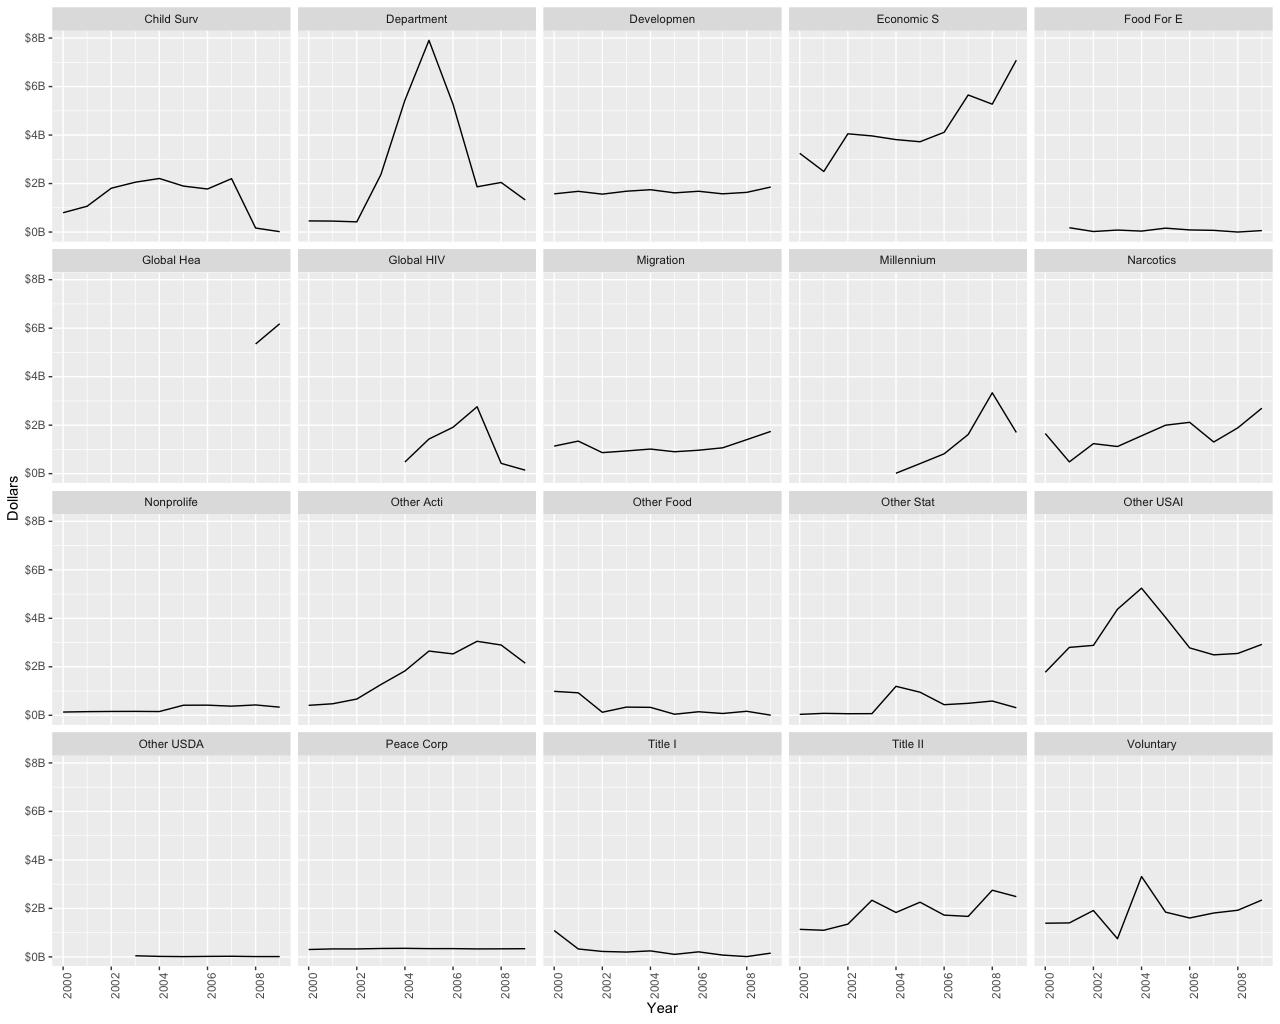
\includegraphics[width=1.0\linewidth]{pic0029}
  \caption{Разход на пари по програми и години}
\label{figure0029}
\end{figure}
\FloatBarrier

Така организирани данните са по редове, за да бъдат трансформирани от редове в колони се използва функцията dcast (Листинг \ref{listing0139}). 

\begin{lstlisting}[caption=От редове към колони, label=listing0139]
melt00 <- melt(Aid_00s, id.vars=c("Country.Name", "Program.Name"), variable.name="Year", value.name="Dollars")
 
 
cast00 <- dcast(melt00, Country.Name + Program.Name ~ Year, value.var="Dollars")
\end{lstlisting}

Първият аргумент на функцията dcast са данните, които да бъдат използвани. Вторият аргумент е формула на която лявата страна са колоните, които трябва да останат колони. От дясната страна са имената, които трябва да станат колони. Третият аргумент е колоната, която трябва да се използва за попълване на данните в новопоявилите се колони. 

\section{Сложни сливания на данни и трансформация на форматите}

Към вече описаните функции за реорганизация на данните се добавят и функциите от пакетите dplyr и tidyr, които позволяват използването на поточни операции. В някои случаи тези функции имат по-добро бързодействие от предходните. 

\subsection{Привързване на редове и колони}

В пакета dplyr привързването на редове и колони се осъществява с функциите bind\_rows и bind\_cols (Листинг \ref{listing0140}). Тези функции са проектирани да работят с data.frame и tibble обекти. Не могат да работят с вектори и матрици. 

\begin{lstlisting}[caption=Обединяване по колони и редове, label=listing0140]
library(dplyr)
library(tibble)

ds1 <- bind_cols(tibble(TV=c("BNT","bTV","Nova"),Channel=c("1","2","3")), tibble(Rating=c("0.1","0.3","0.2")))

ds2 <- tribble(~TV, ~Channel, ~Rating, "HBO", "4", "0.4", "VH1", "5","0.5", "MTV","6", "0.6")

bind_rows(ds1, ds2)
\end{lstlisting}

И двете функции могат да работят с множество от обекти, едновременно.

\subsection{Сложни сливания на данни}

Пакетът dplyr предлага група от функции за извършване на сливания (joins). В множеството данни за диамантите цветът се отбелязва само с една латинска буква, без да има допълнителна информация за значението на самата маркировка. Допълнителна информация за цветовете на диамантите е налична в друго множество от данни, което е много подходящо за демонстрация на сливания между множества данни (Листинг \ref{listing0141}).

\begin{lstlisting}[caption=Сложни сливания, label=listing0141]
library(ggplot2)
library(readr)
library(dplyr)

colors <- as_tibble(read.table("https://raw.githubusercontent.com/TodorBalabanov/Statistical-Data-Processing-with-R/master/data/colors.csv", header=TRUE, sep=","))

left_join(diamonds, colors, by=c('color'='Color')) %>% select(carat, color, price, Description, Details)

tail(right_join(diamonds, colors, by=c('color'='Color')))

inner_join(diamonds, colors, by=c('color'='Color'))

semi_join(colors, diamonds, by=c('Color'='color'))

anti_join(colors, diamonds, by=c('Color'='color'))
\end{lstlisting}

При лявото сливане (left join) данните за диамантите са отляво, а данните за цвета са от дясно. Тъй като колоната използвана за ключ се различава в главно и малко C, то ключът се задава с аргумента by. Данните се подават като вектор, където имената на елементите са колоните в лявата таблица, а стойностите са колоните от дясната таблица. При разминаване на типовете за колоните използвани като ключови (фактори със символни низове), то автоматично се прави преобразуване. При лявото сливане участват всички редове от лявата таблица и само редовете, които отговарят по ключ от дясната таблица. 

При десните сливания (right join) участват всички редове от дясната таблица, дори и когато няма съответствие по ключа в лявата таблица. При използвания пример, това води до поява на редове съдържащи липсващи стойности (NA), там където няма съответствие.

При вътрешното сливане (inner join) участват само редове, които имат съответствие по ключа и в двете таблици. 

При външното сливане (outer join) участват всички редове и от двете таблици, без значение дали имат съответствие по ключа.

В SQL базите данни няма директен еквивалент, но в R има полусливане (semi join), смисълът на което е, че се всеки ред от лявата таблица се връща първото срещане в дясната таблица. По-своята същност това е филтриране по редове. Връщат се само редове, които отговарят на съответствие по ключ. 

Противоположното действие на полусливането в R се постига с anti join. Смисълът е, че се връщат тези редове от лявата таблица, които нямат съответствие по ключ в дясната таблица. 

\subsection{Реформатиране на данните}

Размяната на колони с редове и обратното бе демонстрирана с функциите melt и dcast. Подобна реорганизация по редове и колони може да се постигне с функциите gather и spread от пакета tidyr. 

\begin{lstlisting}[caption=Данни за реакциите, label=listing0142]
library(readr)

emotions <- read_tsv("https://raw.githubusercontent.com/TodorBalabanov/Statistical-Data-Processing-with-R/master/data/reaction.txt")
Parsed with column specification:
cols(
  ID = col_integer(),
  Test = col_integer(),
  Age = col_double(),
  Gender = col_character(),
  BMI = col_double(),
  React = col_double(),
  Regulate = col_double()
\end{lstlisting}

За демонстрация на трансформацията от колони към редове е използвано множеството данни от Columbia University, което изследва емоционалните реакции и задръжки (Листинг \ref{listing0142}). Тъй като данните са в обикновен текстов файл и като разделител се използва символа за табулация, за тяхното прочитане се използва функцията read\_tsv (Tab Separated Values). Данните се зареждат в tibble обект, като за всяка колона се избира подходящ тип данни. 

\begin{lstlisting}[caption=Свиване от колони в редове, label=listing0143]
library(tidyr)

emotions %>% gather(key=Type, value=Measurement, Age, BMI, React, Regulate)

gather(emotions, key=Type, value=Measurement, -ID, -Test, -Gender)
\end{lstlisting}

Данните за емоциите са организирани на колони (wide format). С функцията gather част от колоните са трансформирани в редове (long format). При събирането на данните, за всяко наблюдавано лице, измерванията са записани в следните четири колони Age, BMI, React и Regulate. Така оформени данните са неподходящи за някои видове пресмятания и поради тази причина е разумно четирите вида измервания да бъдат в една колона (Measurement), а втора колона (Type) да показва за кой тип измерване е стойността (Листинг \ref{listing0143}). С функцията gather се получава своеобразно събиране на стойностите от няколко колони в една. Първият аргумент е множеството данни, вторият аргумент ключът за новосъздадената колона, следва колоната със стойностите и след това се изброяват колоните, които формират общата колона със стойности. В оригиналните данни идентификаторът на изследвания обект присъства на два реда (два проведени експеримента), а в трансформираните данни идентификаторът на изследвания обект присъства на осем реда, тъй като за всеки експеримент са добавени по четири реда за различните видове измервания. Възможно е да се направи същата трансформация с изрично изброяване на колоните, които не трябва да бъдат събирани. Тогава се използва символът тилда пред имената на колоните. 

\begin{lstlisting}[caption=Разпъване от редове в колони, label=listing0144]
library(dplyr)

emotions %>% gather(key=Type, value=Measurement, Age, BMI, React, Regulate) %>% arrange(ID)

emotions %>% spread(key=Type, value=Measurement)
\end{lstlisting}

Обратното действие на събирането е разпъване в колони и в пакета tidyr то се постига с функцията spread (Листинг \ref{listing0144}). Аргументът key определя имената на колоните които ще бъдат създадени. Аргументът value определя кои стойности ще бъдат използвани за попълване на новосъздадените колони. 

\section*{Заключение}

